\documentclass[10pt,twocolumn]{article}

\usepackage[margin=0.65in]{geometry}
\usepackage{graphicx}
\usepackage{booktabs}
\usepackage{multirow}
\usepackage{array}
\usepackage[table]{xcolor}
\usepackage{microtype}
\usepackage{amsmath}
\usepackage{caption}
\usepackage{subcaption}
\usepackage{float}
\usepackage[section]{placeins}
\usepackage[hidelinks]{hyperref}

\captionsetup{font=small}
\graphicspath{{outputs/plots/}{plots/}}
\setlength{\columnsep}{0.24in}
\setlength{\textfloatsep}{8pt plus 2pt minus 2pt}
\setlength{\floatsep}{6pt plus 2pt minus 2pt}
\setlength{\intextsep}{6pt plus 2pt minus 2pt}
\setlength{\abovecaptionskip}{4pt}
\setlength{\belowcaptionskip}{0pt}
\renewcommand{\refname}{References}
\definecolor{inlinecodebg}{RGB}{238,238,238}
\let\originaltexttt\texttt
\renewcommand{\texttt}[1]{%
  \begingroup
  \setlength{\fboxsep}{1.2pt}%
  \colorbox{inlinecodebg}{\originaltexttt{#1}}%
  \endgroup
}

\title{\textbf{\Huge TECH REPORT}\\[4pt]
\Large ECG-Only Brugada Syndrome Screening on Brugada-HUCA\\
\Large Using Transfer Learning, ResNet-1D, and\\
\Large Safety-Oriented Model Selection Framework}
\author{\textbf{Team VZ}\\[3pt]Izzar Suly Nashrudin and Risma Muslimah}
\date{}

\begin{document}
\maketitle

\begin{abstract}
This project benchmarks ECG-driven machine learning and deep learning models for binary Brugada syndrome screening on the Brugada-HUCA dataset. We deliberately use an ECG-only primary benchmark to avoid shortcut learning from metadata such as \texttt{basal\_pattern} and \texttt{sudden\_death}. After excluding seven label-2 atypical cases, the final binary benchmark contains 356 patients (287 Normal, 69 Brugada), evaluated with one shared patient-level split across 11 models. The best aggregate model is an in-domain transfer-learning pipeline (PR-AUC 0.694, F1 0.696), while the best safety-oriented model is a ResNet-1D median-beat classifier with higher sensitivity (0.643 vs.\ 0.571) and one fewer false negative. Interpretability analyses consistently highlight right precordial information, especially V1--V3, which is clinically plausible for Brugada syndrome. We position the resulting system as research-stage decision support rather than autonomous diagnosis.
\end{abstract}

\section{Problem Statement and Dataset Justification}
The task is to distinguish Brugada syndrome from Normal 12-lead ECG recordings while balancing two competing goals: strong aggregate discrimination and low false-negative risk. In this setting, missing a true Brugada case is more clinically costly than generating an additional false alarm, so leaderboard performance alone is not sufficient.

Brugada-HUCA is appropriate for this challenge because it directly provides short 12-lead ECGs for a Brugada-focused cohort in WFDB format, enabling end-to-end signal modeling, feature engineering, and clinically grounded interpretability. The repository-level checks confirmed that the recordings are standardized at 100 Hz, 12 seconds, and 12 leads for all indexed subjects. The metadata file contains 363 subjects in total: 287 Normal, 69 confirmed Brugada (\texttt{brugada}=1), and 7 atypical/other cases (\texttt{brugada}=2). Because the competition problem is binary Brugada-vs-Normal classification, we excluded the seven label-2 cases and evaluated the models on a clean 356-patient binary cohort.

\begin{table}[!t]
\centering
\caption{Benchmark cohort and split summary.}
\label{tab:dataset}
\small
\begin{tabular}{lr}
\toprule
Item & Value \\
\midrule
Subjects in metadata & 363 \\
Excluded atypical label-2 cases & 7 \\
Binary benchmark subjects & 356 \\
Normal / Brugada & 287 / 69 \\
Train / Validation / Test & 227 / 57 / 72 \\
Brugada cases in test split & 14 \\
ECG-only feature count & 357 \\
Median-beat tensor shape & $70 \times 12$ \\
\bottomrule
\end{tabular}
\end{table}

The main comparison excludes metadata such as \texttt{basal\_pattern} and \texttt{sudden\_death} so that the reported benchmark remains ECG-driven, fair, and clinically defensible. Metadata is discussed only as a supplementary ablation because it can improve apparent performance without proving better ECG understanding.

\section{Methodology}
Our pipeline follows one shared patient-level stratified split for every model so that comparisons remain fair. We first verified ECG availability and recording specifications for all patients, then loaded each record from WFDB and standardized the lead order to the conventional 12-lead layout.

\textbf{Preprocessing.} Each ECG was filtered with a third-order zero-phase Butterworth band-pass filter from 0.5--40 Hz, then normalized with robust median/MAD scaling. R-peaks were detected from a priority list of reference leads (II, V2, V1, V3, I) using a smoothed signal plus prominence-aware peak finding. Around each accepted beat, we extracted a window of 0.25 s before and 0.45 s after the R-peak, and the patient representation was formed as the median beat across detected beats. This keeps the core morphology while suppressing transient noise.

\textbf{Feature representations.} We built two ECG representations. The first is a 357-dimensional ECG-only feature table that combines per-lead strip statistics, beat morphology descriptors, right-precordial ST/QRS features, and selected cross-lead correlations. The second is a 12-lead median-beat tensor of shape $70 \times 12$ used by end-to-end sequence models.

\textbf{Model families.} We trained 11 ECG-only models in three families: feature-based models (XGBoost, Random Forest, SVM-RBF, AdaBoost), end-to-end deep models (1D CNN, ResNet-1D, CNN+BiGRU, Transformer Encoder), and advanced/transfer approaches (in-domain denoising-autoencoder transfer learning, VICReg self-supervision, and Echo State Network).

\textbf{Imbalance handling and thresholding.} Because Brugada is the minority class, we used stratified splitting, class-balanced training weights, \texttt{scale\_pos\_weight} for XGBoost, weighted AdaBoost fitting, and evaluation metrics that do not rely on accuracy alone. Probabilistic thresholds were tuned on the validation split, not the test split, by maximizing F1 from the precision-recall operating points. The fixed validation-derived threshold was then applied once to the held-out test set. This is stricter than post hoc test-set threshold selection.

\textbf{Evaluation strategy.} We report both a leaderboard-oriented ranking and a safety-oriented clinical ranking. The first emphasizes PR-AUC, F1, sensitivity, balanced accuracy, and correct Brugada detections. The second prioritizes sensitivity and false-negative control. Because multiple models were compared on a single held-out test split, the leaderboard should be interpreted as a useful benchmark rather than a definitive estimate of out-of-sample superiority.

For reproducibility, the generated benchmark artifacts are organized in the repository under \texttt{outputs/} (leaderboards and logs), \texttt{outputs/predict} (predictions and detailed analysis tables), and \texttt{outputs/plots} (figures used in this report).

\section{Results and Validation}
All 11 candidate models trained successfully on the final pipeline. The aggregate winner and the safety-oriented winner are different, which is clinically important rather than inconvenient: it shows that the model with the best global score is not automatically the best screening narrative.

\begin{table}[!t]
\centering
\caption{Held-out test comparison between the best aggregate model and the best safety-oriented clinical candidate.}
\label{tab:main-results}
\scriptsize
\setlength{\tabcolsep}{2.5pt}
\resizebox{\linewidth}{!}{%
\begin{tabular}{>{\raggedright\arraybackslash}p{0.60in} >{\raggedright\arraybackslash}p{0.90in} c c c c c c c}
\toprule
Track & Model & Thr. & PR-AUC & F1 & Sens. & Spec. & FN & FP \\
\midrule
Aggregate & Transfer Learning (DAE) & 0.594 & 0.694 & 0.696 & 0.571 & 0.983 & 6 & 1 \\
Clinical & ResNet-1D Median Beat & 0.517 & 0.572 & 0.643 & 0.643 & 0.914 & 5 & 5 \\
\bottomrule
\end{tabular}
}
\end{table}

The transfer-learning model leads the aggregate leaderboard because it offers the strongest precision-recall behavior and the cleanest specificity profile. However, the ResNet-1D clinical candidate improves sensitivity by 0.071 and reduces false negatives by one case, at the cost of four additional false positives. For a screening-oriented discussion, this trade-off is acceptable and should be stated explicitly.

A balanced multi-aspect ranking that blends aggregate performance, clinical safety, validation consistency, training effort, and available repeated-split evidence also selected the transfer-learning pipeline, with a composite score of 0.718. This supports using transfer learning as the single-model recommendation while still presenting ResNet-1D as the more defensible low-false-negative screening narrative.

\textbf{Threshold rationale.} The safety-oriented ResNet threshold was selected on the validation split at 0.517. On the held-out test set, that operating point detected 9 of 14 Brugada cases (sensitivity 0.643) and correctly rejected 53 of 58 Normal cases (specificity 0.914). A descriptive threshold scan on the same test predictions shows that lower thresholds can increase sensitivity further, but those analyses are presented only to visualize the trade-off and not to retroactively claim a better final threshold.

\begin{figure}[!t]
\centering
\begin{subfigure}[t]{\linewidth}
    \centering
    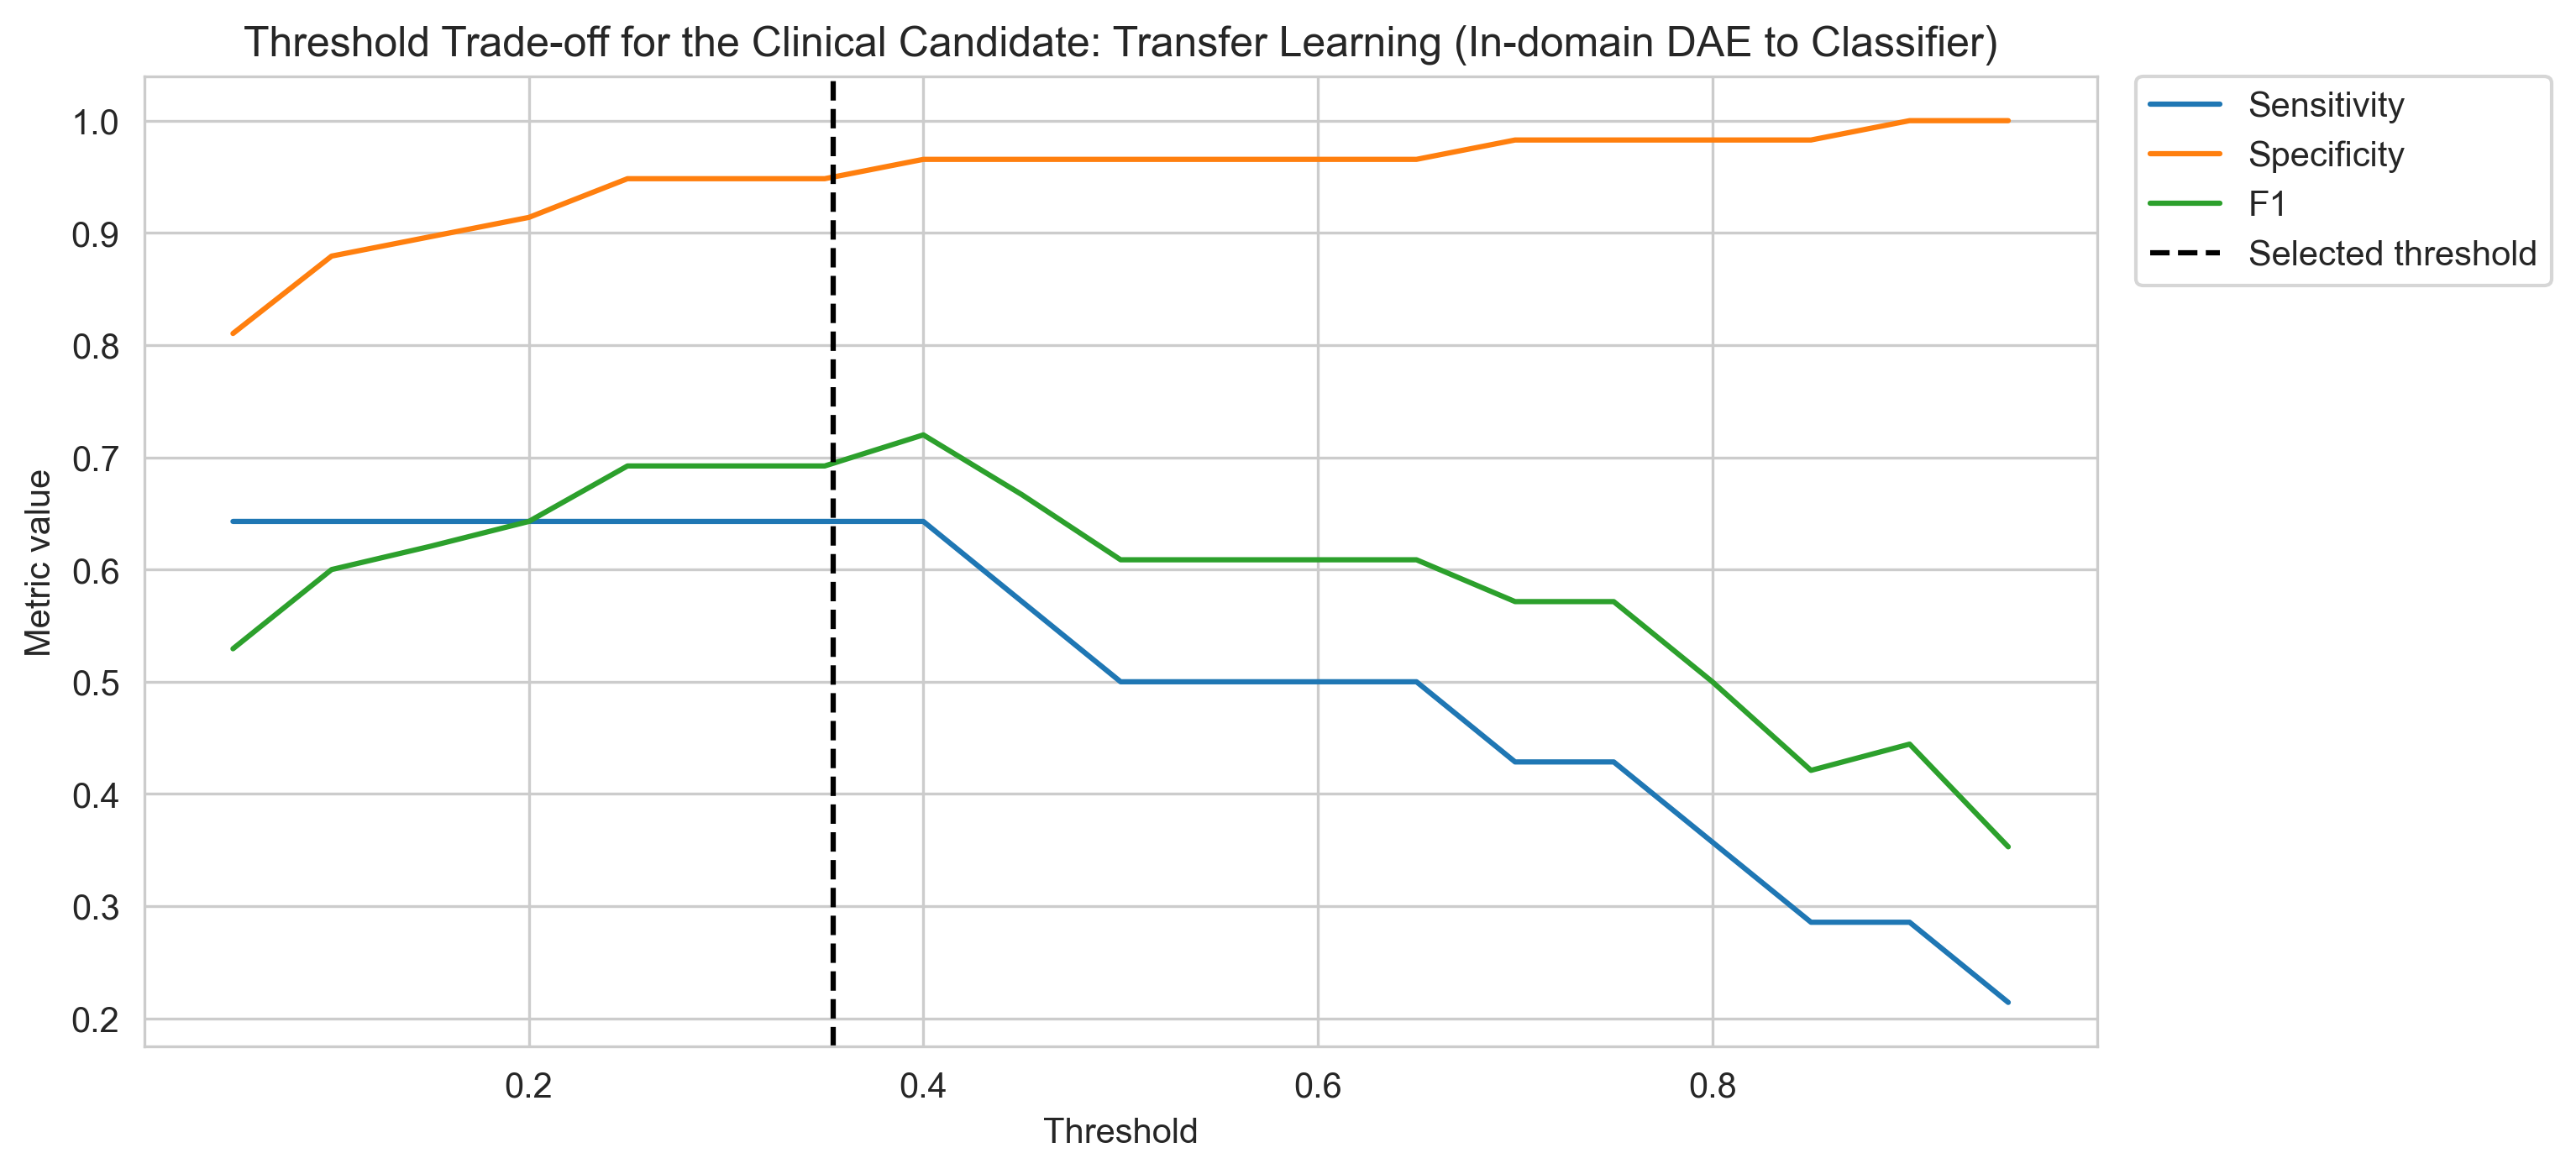
\includegraphics[width=\textwidth]{Failure Analysis Clinical Candidate Threshold Tradeoff.png}
    \caption{Clinical threshold trade-off for the ResNet-1D candidate.}
\end{subfigure}
\vspace{6pt}
\begin{subfigure}[t]{\linewidth}
    \centering
    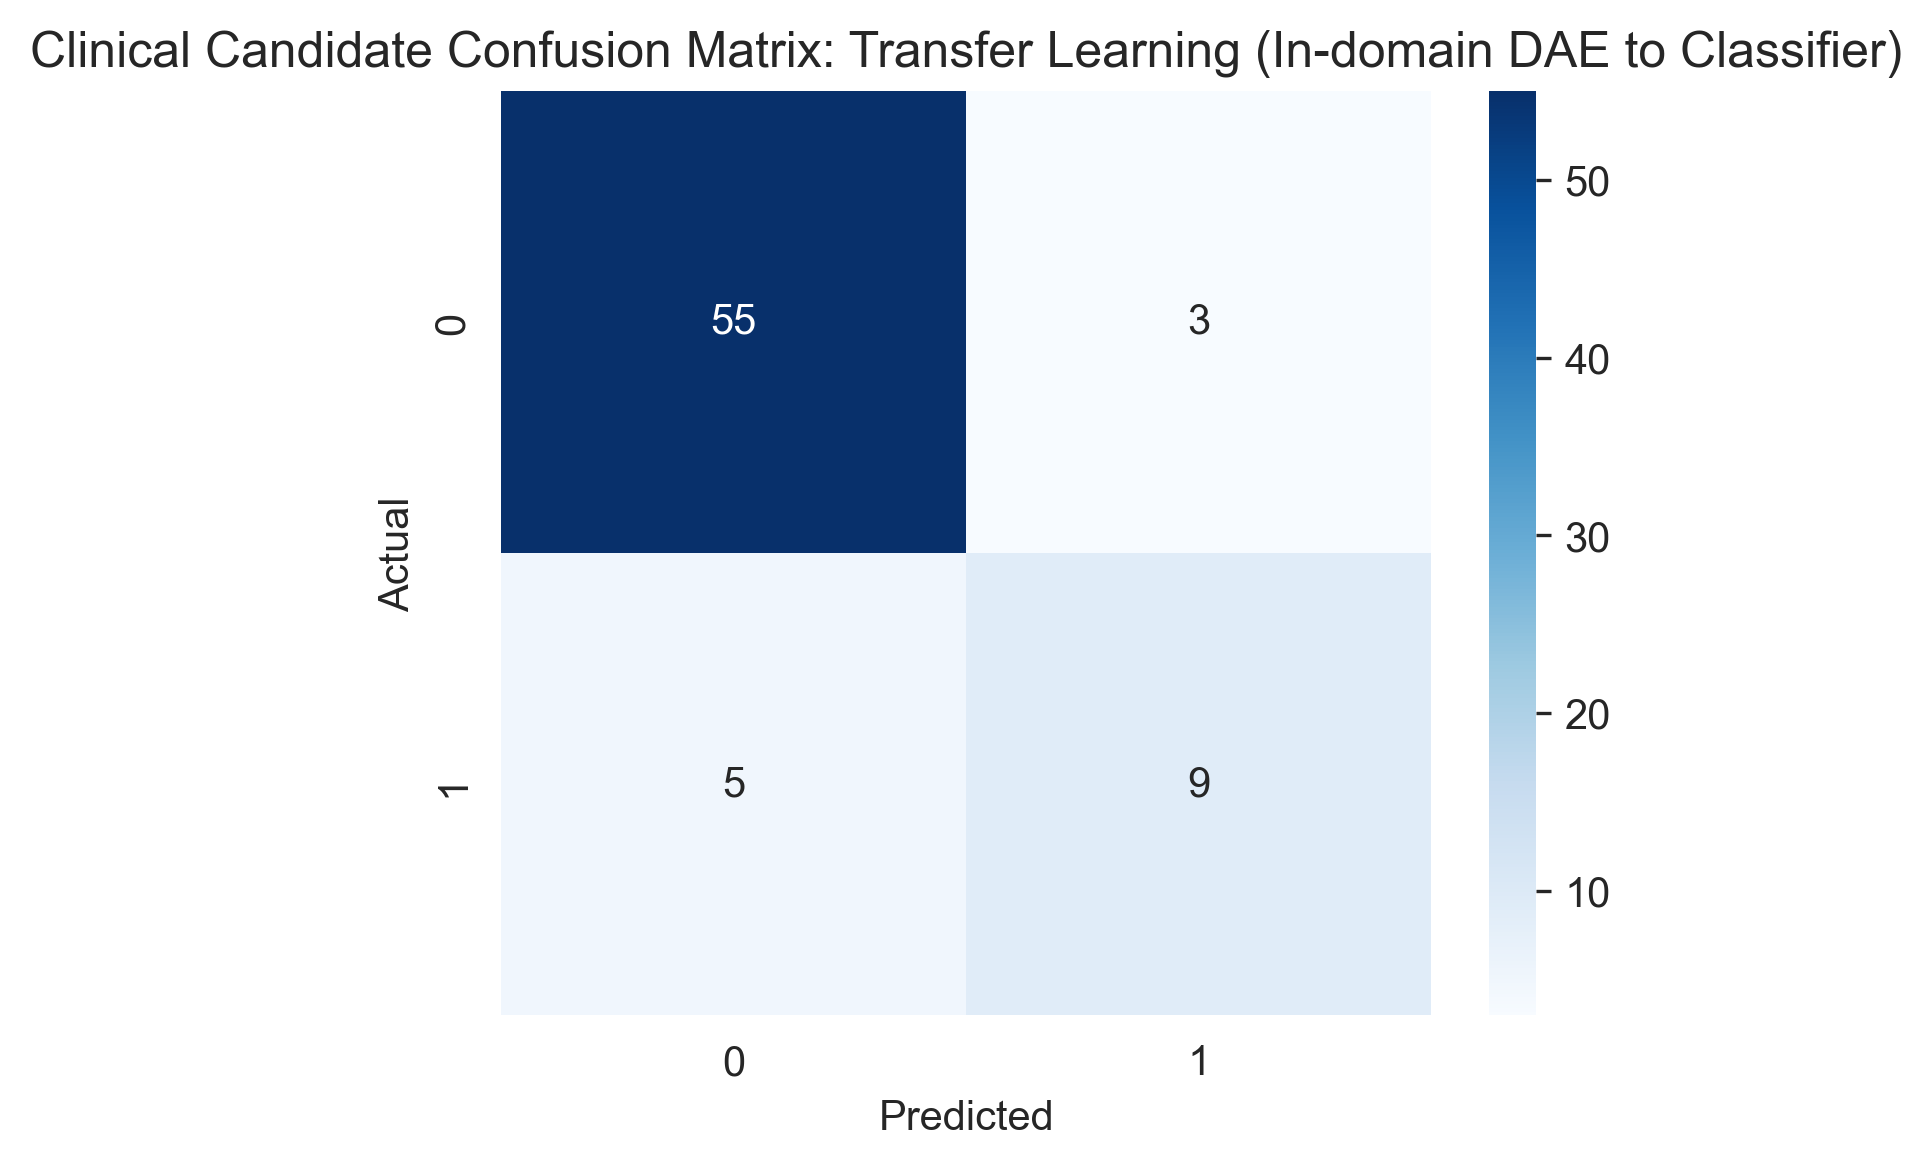
\includegraphics[width=\textwidth]{Validation Clinical Candidate Confusion Matrix.png}
    \caption{Confusion matrix at the validation-derived threshold.}
\end{subfigure}
\caption{Held-out test analysis for the safety-oriented clinical candidate.}
\label{fig:clinical}
\end{figure}

\textbf{Robustness beyond a single split.} To assess stability on a small and imbalanced cohort, we supplemented the shared hold-out benchmark with six repeated patient-level stratified outer splits on the train+validation pool. To keep runtime manageable, this stability check focused on fast ECG-only finalists. The repeated-split summary in Table~\ref{tab:stability} shows that ESN delivered the highest mean sensitivity, whereas XGBoost achieved the strongest mean PR-AUC and the lowest false-negative variance among the tested lightweight models.

\begin{table}[!t]
\centering
\caption{Repeated split stability on the train+validation pool (mean $\pm$ std).}
\label{tab:stability}
\scriptsize
\begin{tabular}{lccc}
\toprule
Model & PR-AUC & Sensitivity & False Negatives \\
\midrule
ESN & $0.535 \pm 0.072$ & $0.619 \pm 0.195$ & $5.33 \pm 2.73$ \\
XGBoost & $0.560 \pm 0.105$ & $0.512 \pm 0.114$ & $6.83 \pm 1.60$ \\
Random Forest & $0.519 \pm 0.119$ & $0.452 \pm 0.224$ & $7.67 \pm 3.14$ \\
\bottomrule
\end{tabular}
\end{table}

This added stability analysis improves rigor, but it does not fully eliminate the model-selection optimism that can arise when many candidate models are compared against one final hold-out split.

\textbf{Metadata ablation.} Adding shortcut-risk metadata produced inconsistent effects: for example, XGBoost sensitivity fell from 0.571 to 0.357, while SVM sensitivity rose from 0.214 to 0.500 with worse specificity. Because these gains are not stable and may reflect shortcut learning rather than stronger ECG reasoning, the main benchmark remains ECG-only.

\section{Interpretability and Clinical Impact}
Interpretability was designed to answer a clinically relevant question: are the models focusing on plausible Brugada regions rather than arbitrary patterns? For the best interpretable feature model (XGBoost), permutation importance aggregated by lead ranked V2 first, followed by V1, with additional contribution from aVF and aVR. Within the right precordial feature set, important variables included \texttt{V2\_minus\_V3\_st\_mean}, \texttt{V1\_strip\_kurtosis}, \texttt{V2\_strip\_max}, and several V1 morphology descriptors. This is compatible with the expectation that Brugada-related morphology is most visible in V1--V3.

For the best safety-oriented sequence model (ResNet-1D), gradient-based lead saliency over the top Brugada-positive test predictions ranked V3 first, with V2 and V1 also among the highest-scoring leads. The V1--V3 heatmap further shows that the network concentrates attention on clinically plausible regions of the median beat rather than distributing it uniformly across all leads and times.

\begin{figure}[!t]
\centering
\begin{subfigure}[t]{\linewidth}
    \centering
    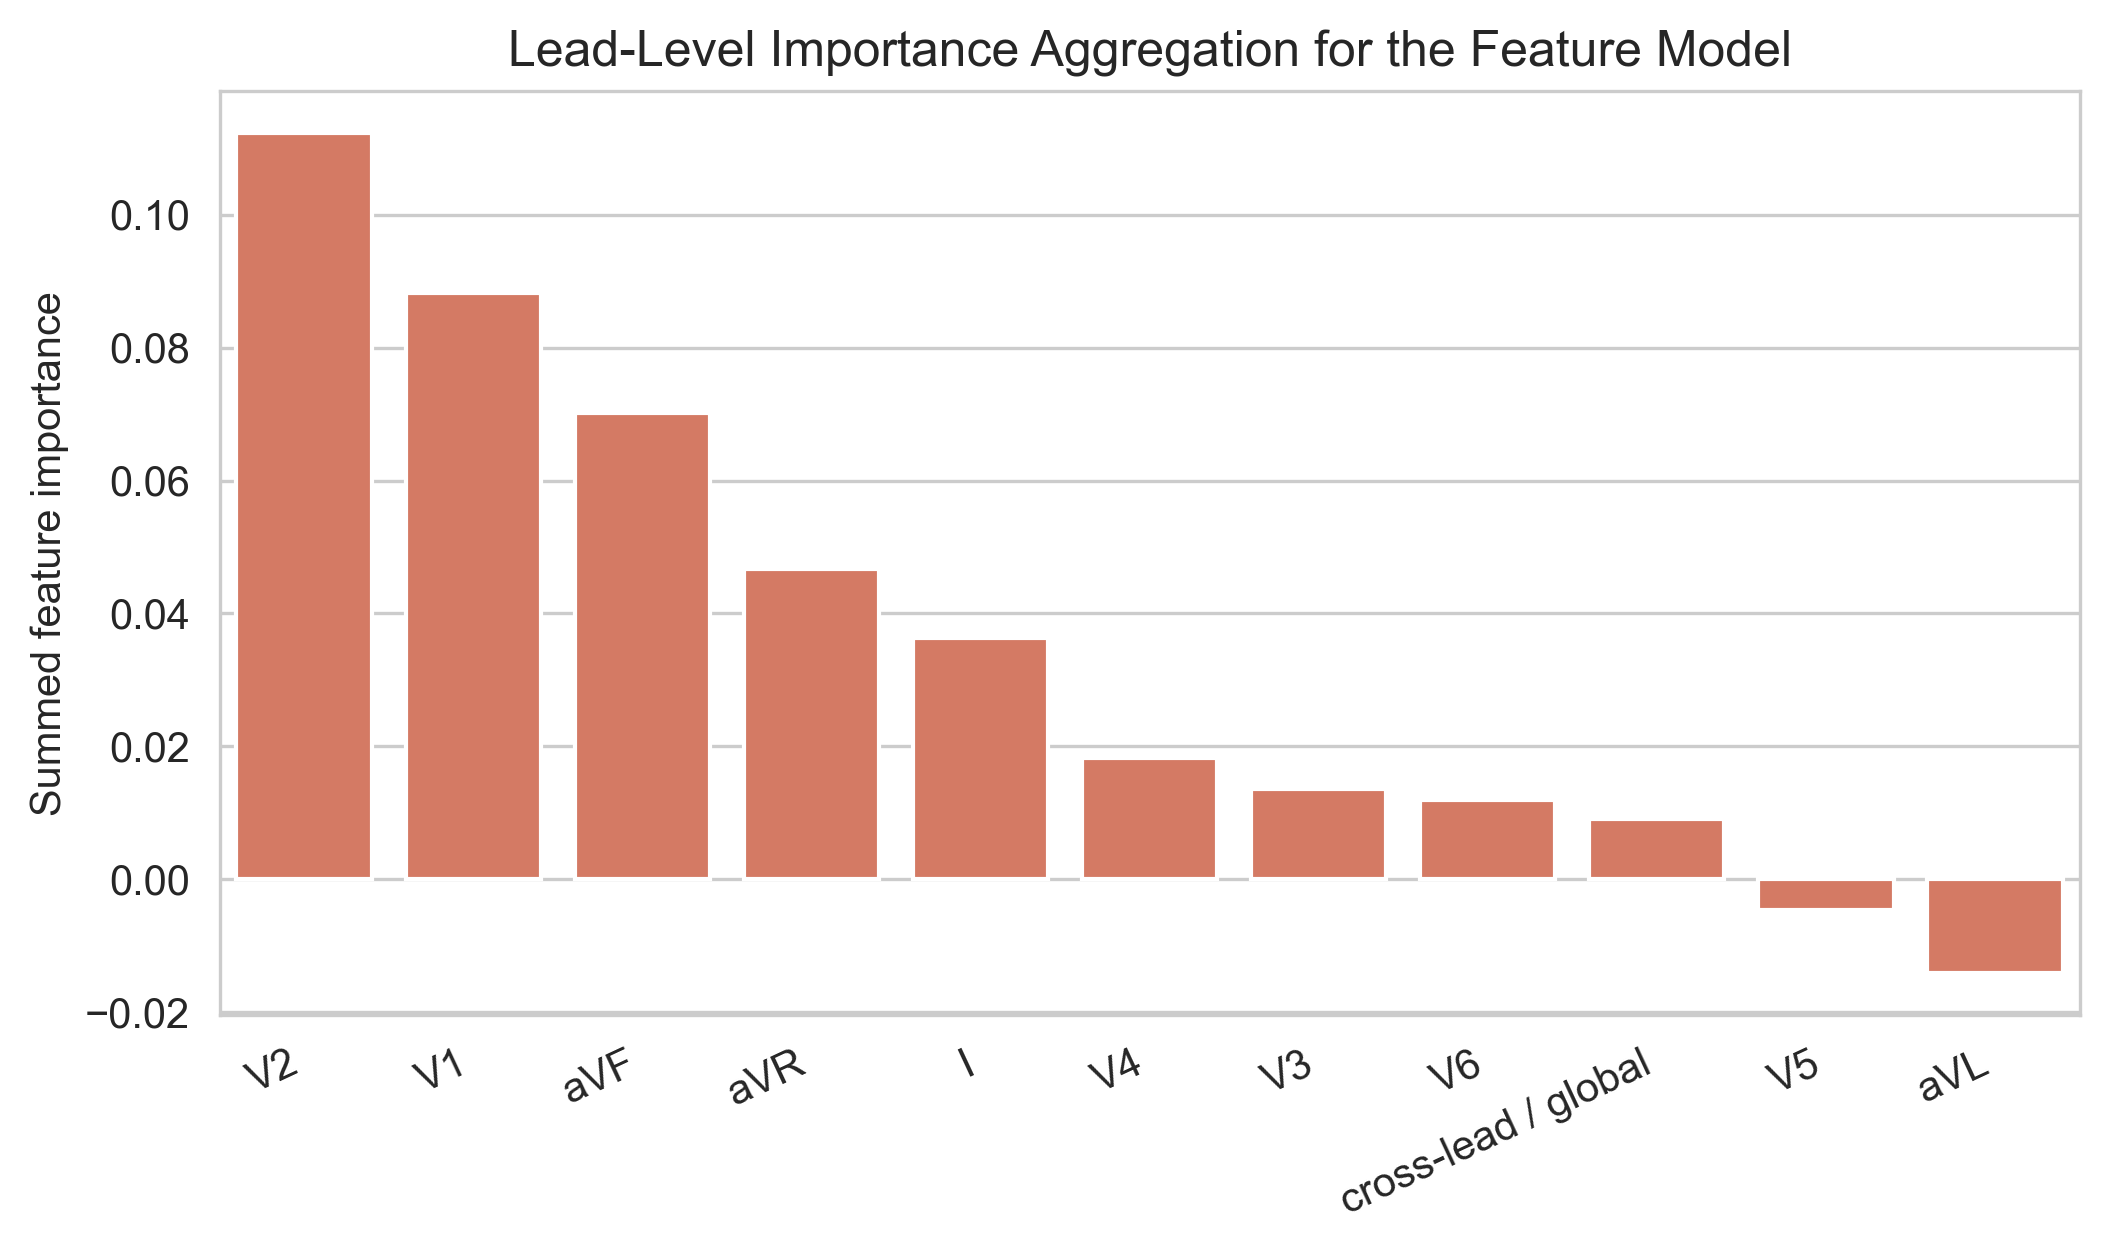
\includegraphics[width=\linewidth]{Interpretability Feature Importance By Lead.png}
    \caption{Lead-level permutation importance from the XGBoost feature model.}
\end{subfigure}
\vspace{4pt}
\begin{subfigure}[t]{\linewidth}
    \centering
    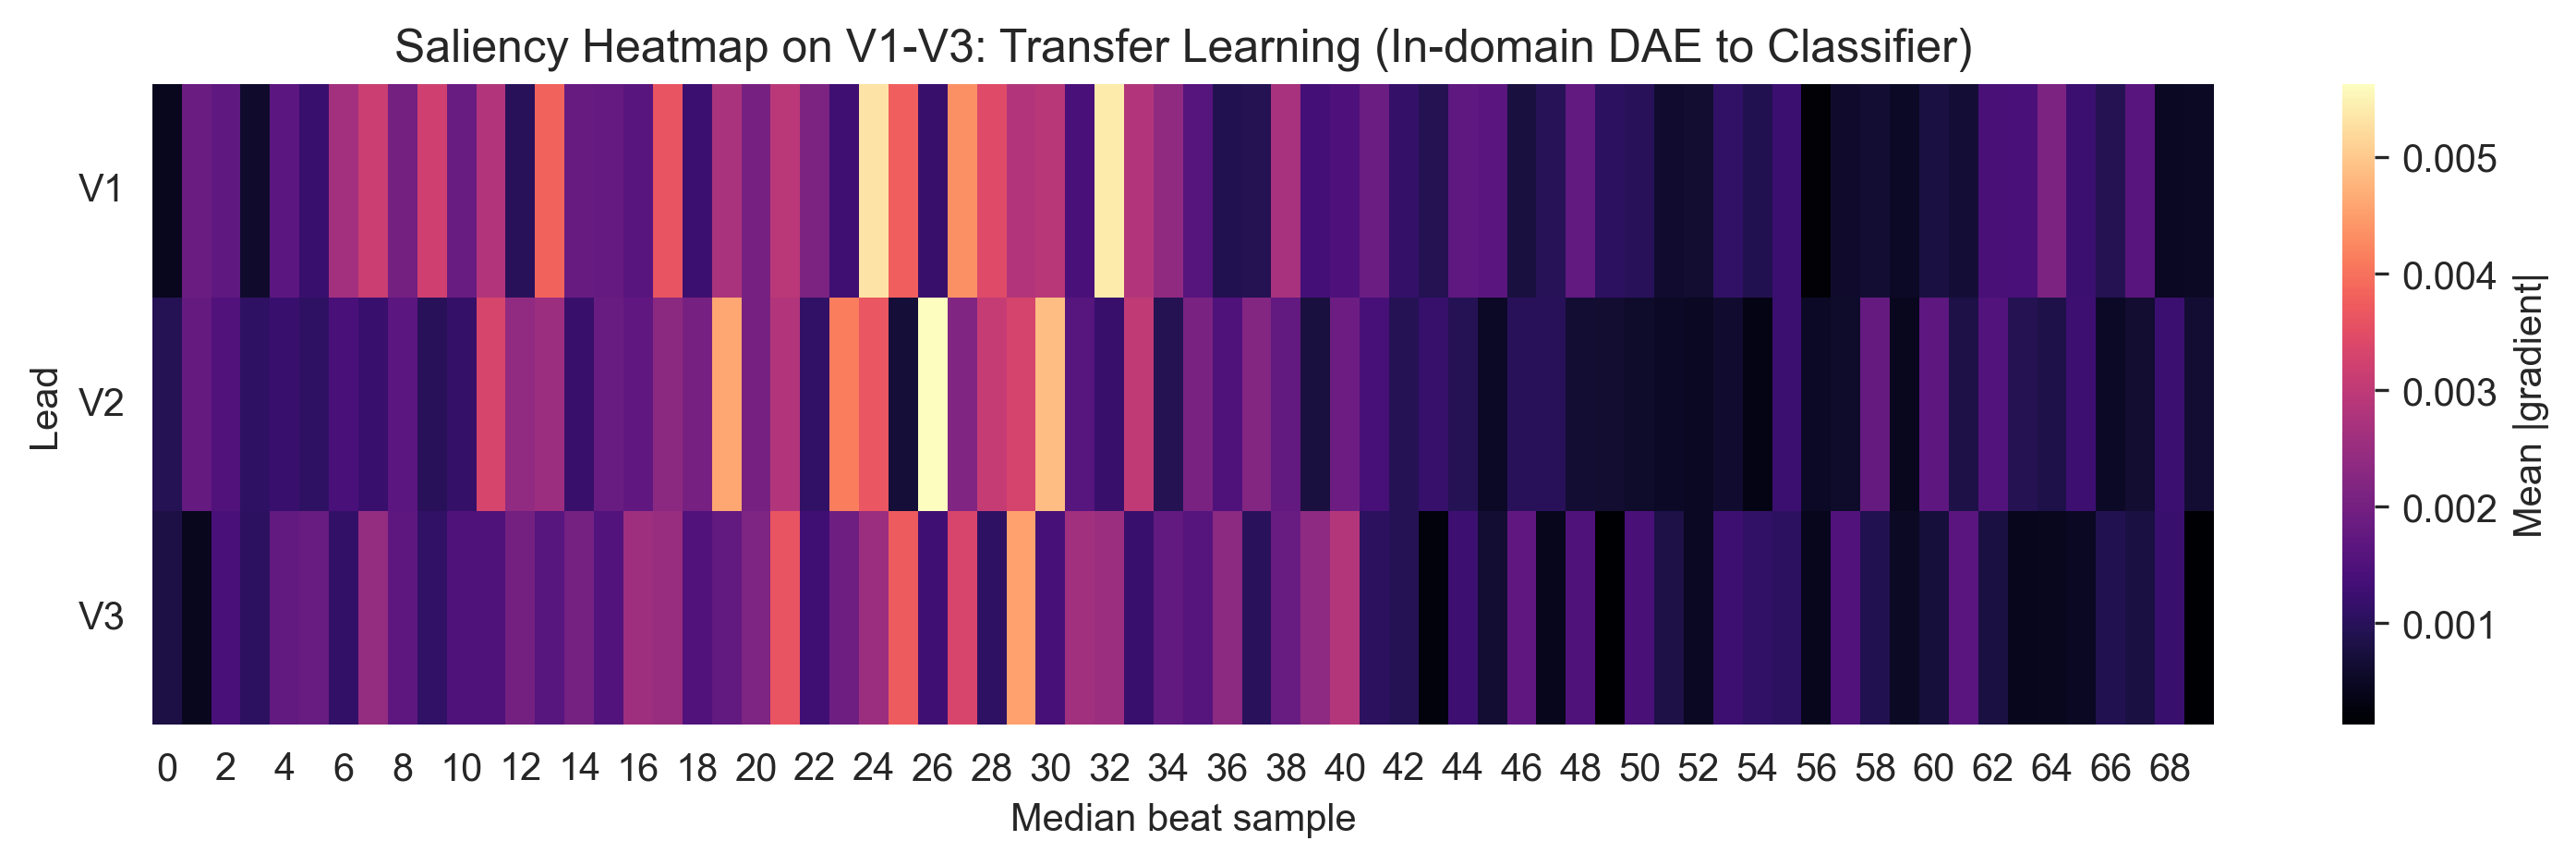
\includegraphics[width=\linewidth]{Interpretability Sequence V1 V3 Saliency Heatmap.png}
    \caption{ResNet-1D saliency heatmap on the clinically relevant V1--V3 leads.}
\end{subfigure}
\caption{Interpretability outputs consistently highlight right precordial information.}
\label{fig:interpretability}
\end{figure}

These interpretability outputs should be read as descriptive transparency tools. They help assess whether the model is focusing on clinically plausible ECG regions, but they do not prove causal reasoning or guarantee safe deployment.

From a clinical workflow perspective, the ResNet-1D candidate is the better screening story because it catches more Brugada cases than the aggregate winner. However, it still leaves 5 false-negative Brugada cases and adds 5 false positives on the test set. Therefore, the current model is better framed as a triage aid or second-reader signal for specialist review, not as an autonomous diagnostic system.

\section{Limitations and Responsible Deployment}
This study has several important limitations. First, the cohort is small and imbalanced, and the benchmark is based on a single dataset without external validation. Second, the binary setup excludes seven atypical label-2 subjects, which simplifies the real diagnostic spectrum. Third, repeated split analysis was limited to lightweight finalists for runtime reasons, so deep-model stability remains an open question. Fourth, many candidate models were compared on one held-out test split, which introduces selection optimism even when the split itself is untouched during threshold tuning.

For responsible deployment, any future system should undergo external validation, prospective operating-point calibration, subgroup analysis, and workflow design that clearly assigns final authority to clinicians. In short, the present results show promise for interpretable ECG-based decision support, but they are not sufficient for standalone diagnosis.
\newpage
\begin{thebibliography}{9}
\bibitem{brugadahuca}
N. Costa Cortez and D. Garcia Iglesias, ``Brugada-HUCA: 12-Lead ECG Recordings for the Study of Brugada Syndrome,'' version 1.0.0, PhysioNet, 2026, RRID:SCR\_007345. doi: \href{https://doi.org/10.13026/0m2w-dy83}{10.13026/0m2w-dy83}.

\bibitem{physionet}
A. Goldberger, L. Amaral, L. Glass, J. Hausdorff, P. C. Ivanov, R. Mark, et al., ``PhysioBank, PhysioToolkit, and PhysioNet: Components of a new research resource for complex physiologic signals,'' \emph{Circulation}, vol. 101, no. 23, pp. e215--e220, 2000, RRID:SCR\_007345. doi: \href{https://doi.org/10.1161/01.CIR.101.23.e215}{10.1161/01.CIR.101.23.e215}.
\end{thebibliography}

\end{document}
